\documentclass[aspectratio=169]{beamer}



%% Full theme: AnnArbor Antibes Bergen Berkeley Berlin Boadilla boxes CambridgeUS Copenhagen Darmstadt default Dresden EastLansing Frankfurt Goettingen Hannover Ilmenau JuanLesPins Luebeck Madrid Malmoe Marburg Montpellier PaloAlto Pittsburgh Rochester Singapore Szeged Warsaw
% \usetheme{Luebeck}

%% outer themes (header/footer): default infolines miniframes smoothbars sidebar split shadow tree smoothtree
% \useoutertheme[subsection=false]{smoothbars}
% \usetheme{Rochester}
\useoutertheme{split}

%% inner theme (content): default circles rectangles rounded inmargin
\useinnertheme{rectangles}

\usecolortheme{beaver}

\usepackage{esvect}

\input{style}


\definecolor{forestgreen}{rgb}{0.0, 0.50, 0.13}

\definecolor{okitho}{HTML}{e69f00}
\definecolor{okitor}{HTML}{d55e00}
\definecolor{okitye}{HTML}{f0e442}
\definecolor{okitcy}{HTML}{56b4e9}
\definecolor{okitgr}{HTML}{009e73}
\definecolor{okitbl}{HTML}{0072b2}
\definecolor{okitpi}{HTML}{cc79a7}

\definecolor{tolbrpi}{HTML}{ee6677}
\definecolor{tolbrgr}{HTML}{228833}
\definecolor{tolbrbl}{HTML}{4477aa}
\definecolor{tolbrye}{HTML}{ccbb44}
\definecolor{tolbrcy}{HTML}{66ccee}
\definecolor{tolbrpu}{HTML}{aa3377}
\definecolor{tolbrgy}{HTML}{bbbbbb}

\definecolor{mypurp}{HTML}{8f0c97}
\definecolor{myred}{HTML}{9f103b}
\definecolor{myor}{HTML}{ae3011}
\definecolor{mydarkor1}{HTML}{96240f}
\definecolor{mydarkor2}{HTML}{7f180c}
\definecolor{mylb1}{HTML}{00557e}
\definecolor{mylb2}{HTML}{013157}
\definecolor{mylb2}{HTML}{013157}
\definecolor{mybl1}{HTML}{0d08a9}
\definecolor{mybl2}{HTML}{04037f}
\definecolor{mygr1}{HTML}{097e3e}
\definecolor{mygr2}{HTML}{025520}
\input ./avanzi-tikz-defs.tex

\definecolor{tolmupu}{HTML}{882255}

\usetikzlibrary{fit,decorations.pathreplacing,decorations.pathmorphing, snakes, intersections}

%%% vectors in bold
\newcommand{\word}[1]{\ensuremath{\boldsymbol{#1}}}
\newcommand{\av}{\word{a}} \newcommand{\cv}{\word{c}}
\newcommand{\bv}{\word{b}} \newcommand{\ev}{\word{e}}
\newcommand{\rv}{\word{r}} \renewcommand{\vv}{\word{v}}
\newcommand{\xv}{\word{x}} \newcommand{\kv}{\word{k}}
\newcommand{\uv}{\word{u}} \newcommand{\Xv}{\word{X}}
\newcommand{\wv}{\word{w}} \newcommand{\rt}{\mathrm{rt}}
\newcommand\p{{\textcolor{purple}{p}}}
\newcommand\q{{\textcolor{purple}{q}}}
\newcommand\lambdorange{{\textcolor{mydarkor1}{\lambda}}}
\newcommand\Wider[2][3em]{%
  \makebox[\linewidth][c]{%
    \begin{minipage}{\dimexpr\textwidth+#1\relax}
      \raggedright#2
    \end{minipage}%
  }%
}
\newtheorem{proposition}{Useful Proposition}
\newtheorem{exemple}{Example}
\usepackage[outline]{contour}




\defcolvar{a}{a}{red}
\defcolvar{b}{b}{brown}


\title{Algebraic Attacks: Theoretical Aspects}
\author{Aurélien Bœuf,\inst{1} Léo Perrin\inst{1}}

\institute{\inst{1}Inria, France}

\begin{document}

\maketitle

\begin{frame}{In this Presentation}
  \begin{center}
    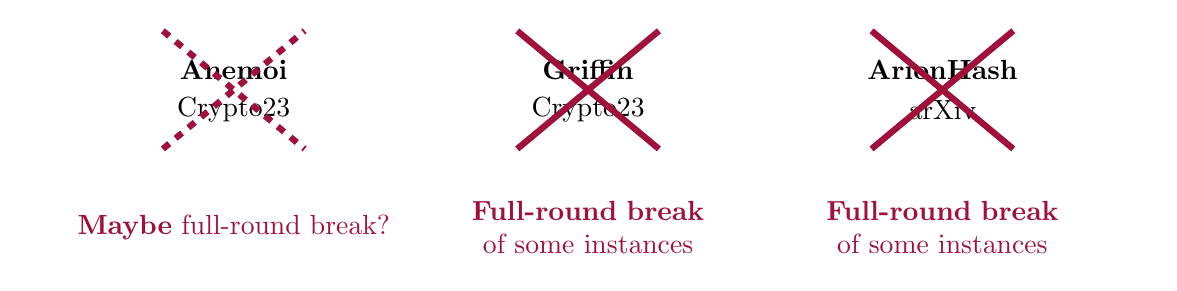
\begin{tikzpicture}[ultra thick,xscale=.9]
      \node (A1) at (0,0) {\bf Anemoi};
      \node (A2) at (0,-.5) {Crypto23};
      \node (B1) at (5,0) {\bf Griffin};
      \node (B2) at (5,-.5) {Crypto23};
      \node (C1) at (10,0) {\bf ArionHash};
      \node (C2) at (10,-.5) {arXiv};

      \pause
      \draw[line width=.8mm, color=myred] (4,-1) -- (6,.5);
      \draw[line width=.8mm, color=myred] (4,.5) -- (6,-1);
      \node[text width=5cm, align=center] (D2) at (B2 |- 5,-2) {\textcolor{myred}{\textbf{Full-round break} of some instances}};
      
      \pause
      \draw[line width=.8mm, color=myred] (9,-1) -- (11,.5);
      \draw[line width=.8mm, color=myred] (9,.5) -- (11,-1);
      \node[text width=5cm, align=center] (D3) at (C2 |- 5,-2) {\textcolor{myred}{\textbf{Full-round break} of some instances}};

      \pause
      \draw[line width=.8mm, color=myred, dashed] (-1,-1) -- (1,.5);
      \draw[line width=.8mm, color=myred, dashed] (-1,.5) -- (1,-1);
      \node[text width=5cm, align=center] (D1) at (A2 |- 5,-2) {\textcolor{myred}{\textbf{Maybe} full-round break?}};
    \end{tikzpicture}
  \end{center}

  \pause\vspace{1cm}
  \onslide<5->{
    \begin{center}
      { \Large How did this happen? }      
    \end{center}
  }
\end{frame}



\tocStartsAppearingHere{}

\section{Cryptanalysis as a Root-Finding Problem}


\begin{frame}{Algebraic Attack? What is that?}
  \vfill

  \begin{center}
    \includegraphics[width=8cm]{./figures/simpsons}
  \end{center}
  
  \vfill
\end{frame}


\begin{frame}{Pipeline of a Root-Finding Attack}

  \begin{enumerate}
    \setlength\itemsep{0.4cm}
  \item Design an attack \pause
  \item Write a (system of) equation(s) \pause
  \item \alert{???} \pause
  \item Deduce a preimage/CICO solution/master key...
  \end{enumerate}

  \pause\vspace{0.4cm}

  \begin{center}
    { \large
      The topic of this class: the ``\alert{???}'' part!
    }      
  \end{center}
\end{frame}



\subsection{A Simple Case: CICO against Feistel-MiMC}


\begin{frame}{Let's Look at Feistel-MiMC}
  \vfill

  \begin{center}
    \includegraphics[width=8cm]{./figures/simpsons}
  \end{center}
  
  \vfill
\end{frame}


\subsection{The Multi-Variate Case}


\begin{frame}{Deriving a Multi-Variate System: CICO-2}
  \vfill

  \begin{center}
    \includegraphics[width=8cm]{./figures/simpsons}
  \end{center}
  
  \vfill
\end{frame}


\section{Introduction to Gröbner Bases}

\subsection{Very High Level View}

\begin{frame}{Root Finding: Simple Cases}

  \begin{overprint}
    \only<1>{

      Consider a multivariate polynomial ring $\mathbb{F}[\textcolor{mylb1}{x_1},\textcolor{myor}{x_2},\ldots,\textcolor{myred}{x_N}]$.

      We want to solve:
      \vspace{0.3cm}
      
      \begin{equation*}
        \left\{
          \begin{aligned}
            p_1(\textcolor{mylb1}{x_1},\ldots&,\textcolor{myred}{x_N}) = 0 \\
            p_2(\textcolor{mylb1}{x_1},\ldots&,\textcolor{myred}{x_N}) = 0 \\
            \vdots \\
            p_k(\textcolor{mylb1}{x_1},\ldots&,\textcolor{myred}{x_N}) = 0
          \end{aligned}
        \right.
      \end{equation*}
    }

    \only<2>{

      \begin{equation*}
        \left\{
          \begin{aligned}
            m_{1,1}\textcolor{mylb1}{x_1} + \cdots& + m_{1,N}\textcolor{myred}{x_N} + a_1 = 0 \\
            m_{2,1}\textcolor{mylb1}{x_1} + \cdots& + m_{2,N}\textcolor{myred}{x_N} + a_2 = 0 \\
            \vdots \\
            m_{k,1}\textcolor{mylb1}{x_1} + \cdots& + m_{k,N}\textcolor{myred}{x_N} + a_k = 0
          \end{aligned}
        \right.
      \end{equation*}

      \vspace{0.5cm}
      
      Polynomials of \textbf{degree 1}: Linear system $\Rightarrow$ \textbf{Linear algebra}.
    }

    \only<3>{
      \begin{equation*}
        \left\{
          \begin{aligned}
            p_1(\textcolor{mylb1}{x_1}) &= 0 \\
            p_2(\textcolor{mylb1}{x_1}) &= 0 \\
            \vdots \\
            p_k(\textcolor{mylb1}{x_1}) &= 0
          \end{aligned}
        \right.
      \end{equation*}

      \vspace{0.5cm}
      
      \textbf{One variable}: Univariate root finding $\Rightarrow$ \textbf{Euclidian division} (for Berlekamp-Rabin algorithm).
    }
  \end{overprint}
\end{frame}


\begin{frame}{Root Finding: The Less Simple Case}
  \begin{columns}
    \begin{column}{0.3\textwidth}
      \begin{equation*}
        \left\{
          \begin{aligned}
            p_1(\textcolor{mylb1}{x_1},\ldots,\textcolor{myred}{x_N}) &= 0 \\
            p_2(\textcolor{mylb1}{x_1},\ldots,\textcolor{myred}{x_N}) &= 0 \\
            \vdots \\
            p_k(\textcolor{mylb1}{x_1},\ldots,\textcolor{myred}{x_N}) &= 0
          \end{aligned}
        \right.
      \end{equation*}

      \vspace{0.5cm}
      
      Several variables,

      high degree!
    \end{column}
    \hfill
    \begin{column}{0.65\textwidth}
      \pause

      \begin{exampleblock}{General Approach}
        If $p_i(\textcolor{mylb1}{x_1},\ldots,\textcolor{myred}{x_N}) = 0$ for all $i$, then
        \begin{equation*}
          \sum_i q_i(\textcolor{mylb1}{x_1},\ldots,\textcolor{myred}{x_N})p_i(\textcolor{mylb1}{x_1},\ldots,\textcolor{myred}{x_N}) ~=~ 0,
        \end{equation*}
        for any set of polynomials $\{q_i\}_i$.

        \pause\vspace{0.2cm}

        The set of all such linear combinations is

        the \alert{ideal generated by the $\{p_i\}_{i=1}^{k}$}

        \vspace{0.2cm}
        
        We denote it $I(p_0,...,p_{n-1})$.
      \end{exampleblock}
    \end{column}
  \end{columns}
  \pause\vspace{0.2cm}
  \begin{center}

    {\large \textbf{Goal:} somehow, find a polynomial $r(\textcolor{mylb1}{x_1})=0$ in this ideal!}

  \end{center}
\end{frame}


\subsection{Setting Up a Mathematical Machinery}

\begin{frame}{Using the Ideal Structure}
  \begin{alertblock}{Over the integer}
    There is an ideal you all know: $n\mathbb{Z} = \{ ..., -3n, -2n, -n, 0, n, 2n, 3n, ... \}$.

    \pause

    Every $x \in \mathbb{Z}$ can be written as $\mya + \myb$, where $\mya \in n\mathbb{Z}$ and $\myb \in$ \pause $\mathbb{Z} / n\mathbb{Z}$.
  \end{alertblock}

  \pause

  \begin{center}
    We want to simplify our lives and work in
    \begin{equation*}
      \mathbb{F}[\textcolor{mylb1}{x_1},\textcolor{myor}{x_2},\ldots,\textcolor{myred}{x_N}]  / I(p_0,...,p_{n-1})~.
    \end{equation*}
  \end{center}
  
\end{frame}


\begin{frame}{A Problem with Euclidian Division}
  \only<1-2>{
  \begin{itemize}

  \item Euclidian division on \textbf{integers}:

    \begin{equation*}
      a = bq + r \text{ , \ }0 \le r < b.
    \end{equation*}
    Division of 13 by 3:
    \[ 13 = 4 \times 3 + 1. \]

  \pause
  \item Euclidian division on \textbf{univariate polynomials} ($\mathbb{F}[\textcolor{mylb1}{X}]$):
    \begin{equation*}
      A = BQ + R \text{ , \ deg($R$) < deg($B$).}
    \end{equation*}
    Division of $\textcolor{mylb1}{X}^3 + \textcolor{mylb1}{X} + 1$  by $\textcolor{mylb1}{X}$:
    \begin{equation*}
      \textcolor{mylb1}{X}^3 + \textcolor{mylb1}{X} + 1 = (\textcolor{mylb1}{X}^2 + 1)\textcolor{mylb1}{X} + 1. 
    \end{equation*}
  \end{itemize} 
}

\end{frame}

\begin{frame}
  \frametitle{The Problem with Multivariate}
  \begin{itemize}
  \item Euclidian division on \textbf{multivariate polynomials}:

    \[ A = BQ + R \text{... condition on $R$}? \]

    \pause
    Division of $\textcolor{mylb1}{x}$ by $\textcolor{mylb1}{x} + \textcolor{myor}{y}$ in $\mathbb{F}[\textcolor{mybl2}{x},\textcolor{myor}{y}]$:
    \begin{align*}
      \textcolor{mylb1}{x} = 0 \cdot (\textcolor{mylb1}{x} +& \textcolor{myor}{y}) + \textcolor{mylb1}{x} \onslide<3>{\ \ \ \ \Leftarrow\  \textcolor{mylb1}{x} < \textcolor{myor}{y}}  \\
      or& \\
      \textcolor{mylb1}{x} = 1 \cdot (\textcolor{mylb1}{x} +&\textcolor{myor}{y}) - \textcolor{myor}{y} \onslide<2>{\text{ ?}} \onslide<3>{\ \ \Leftarrow\  \textcolor{myor}{y} < \textcolor{mylb1}{x}}
    \end{align*}

    \pause
    Need to define a \textbf{monomial ordering}.

    $\implies$ Division steps determined by \textbf{leading monomials (LM)}.
  \end{itemize}
  
\end{frame}


\begin{frame}
  \frametitle{Monomial orderings}

  In $\mathbb{F}[\textcolor{mylb1}{x},\textcolor{myor}{y},\textcolor{mypurp}{z}]$:
  \begin{itemize}
  \item \textbf{LEXicographical:} Compare degree of highest variable, then second-highest, etc. 
    \[ \textcolor{mylb1}{x} <_{\text{lex}} \textcolor{myor}{y} <_{\text{lex}} \textcolor{mypurp}{z} \;,\ \ \textcolor{mylb1}{x}^{1000}  \onslide<1>{\ \;?\ }\onslide<2->{\hspace{-1.5em}<_{\text{lex}}} \textcolor{myor}{y} \pause \;,\ \ \textcolor{mylb1}{x}^6 \textcolor{myor}{y} \textcolor{mypurp}{z} \onslide<2>{\ \;?\ }\onslide<3->{\hspace{-1.5em}<_{\text{lex}}} \textcolor{myor}{y}^2 \textcolor{mypurp}{z} \pause \;. \]
  \pause \item \textbf{Graded LEX:} Compare \textbf{total degree} first, then switch to lex if equality.

    \[ \textcolor{mylb1}{x} <_{\text{lex}} \textcolor{myor}{y} <_{\text{lex}} \textcolor{mypurp}{z} \;,\ \ \textcolor{myor}{y} \onslide<4>{\ \ \ ?\ }\onslide<5->{\hspace{-1.8em}<_{\text{glex}}} \textcolor{mylb1}{x}^2 \pause \;,\ \ \textcolor{mypurp}{z}^2 \onslide<5>{\ \ \ ?\ }\onslide<6->{\hspace{-1.8em}<_{\text{glex}}} \textcolor{mylb1}{x}\textcolor{myor}{y}\textcolor{mypurp}{z} \pause \;,\ \ \textcolor{mylb1}{x}\textcolor{myor}{y} <_{\text{glex}} \textcolor{mylb1}{x}\textcolor{mypurp}{z} <_{\text{glex}} \textcolor{myor}{y}\textcolor{mypurp}{z}\;. \]

  \pause \item \textbf{Weighted Graded LEX:} Compare the \textbf{weighted sum} of degrees, then lex if equality. Examples for $\textcolor{mylb1}{x} <_{\text{lex}} \textcolor{myor}{y} <_{\text{lex}} \textcolor{mypurp}{z}$ and $\mathbf{wt}(\textcolor{mylb1}{x}) = 6,  \mathbf{wt}(\textcolor{myor}{y}) = 1, \mathbf{wt}(\textcolor{mypurp}{z}) = 2$:

  \[ \textcolor{mylb1}{x} \onslide<7>{\ \ \ \ \;?\ }\onslide<8->{\hspace{-2em}>_{\text{wglex}}} \textcolor{myor}{y}\textcolor{mypurp}{z}^2 \pause \text{ because }\mathbf{wt}(\textcolor{mylb1}{x})=6 \text{ and }\mathbf{wt}(\textcolor{myor}{y}\textcolor{mypurp}{z})=\mathbf{wt}(\textcolor{myor}{y}) + 2\mathbf{wt}(\textcolor{mypurp}{z}) = 5 \;. \]

  \vspace{-.8cm}
  \[\textcolor{mylb1}{x}^2 \onslide<8>{\ \ \ \ \;?\ }\onslide<9->{\hspace{-2em}<_{\text{wglex}}} \textcolor{mypurp}{z}^6 \pause \text{ because }\mathbf{wt}(\textcolor{mylb1}{x}^2)=\mathbf{wt}(\textcolor{mypurp}{z}^6)=12 \text{ and }\textcolor{mylb1}{x}^2 <_{\text{lex}} \textcolor{mypurp}{z}^6 \;. \]

  \end{itemize}
  
\end{frame}

\begin{frame}
  \frametitle{The Problem... Still.}

  Consider a system $\left\{p_1, \ldots, p_k\right\}$.
  
  $\implies$ Division of a polynomial $p$ by $\left\{p_1, \ldots, p_k\right\}$ for some ordering: \textbf{final remainder can depend on the choice of divisors!}

  \pause

  Example: in $\mathbb{F}[\textcolor{mylb1}{x},\textcolor{myor}{y}]$ with \textbf{lex} ordering ($\textcolor{mylb1}{x} <_{lex} \textcolor{myor}{y}$), divide $\textcolor{myor}{y}^2$ by $\left\{\textcolor{myor}{y}^2 - 1, \textcolor{myor}{y} - \textcolor{mylb1}{x}\right\}$.

  \begin{center}
  \begin{tabular}{cc|cc}
    $\textcolor{myor}{y}^2$ & &\hspace{1cm} $\textcolor{myor}{y}^2$& \\
    $\Big\Downarrow$ & red. by $\textcolor{myor}{y}^2 - 1$ \hspace{1cm} & \hspace{1cm} $\Big\Downarrow$ & red. by $\textcolor{myor}{y} - \textcolor{mylb1}{x}$ \\
    $1$ & &\hspace{1cm} $\textcolor{mylb1}{x}\textcolor{myor}{y}$& \\
    $\Big\Downarrow$ & no further red. \hspace{1cm} & \hspace{1cm} $\Big\Downarrow$ & red. by $\textcolor{myor}{y} - \textcolor{mylb1}{x}$ \\
    $1$ & & \hspace{1cm}$\textcolor{mylb1}{x}^2$ &
  \end{tabular}

\end{center}

\pause

\centering
\textbf{The solution: Gröbner Bases.}
\end{frame}


\begin{frame}
  \frametitle{What is a Gröbner Basis?}


  Let $G = \{p_1,\ldots,p_k\}$ and $<$ a monomial ordering.

  \vspace{0.2cm}

  \begin{definition}
    $G$ is a \emph{Gröbner basis} if and only if the reduction defined by $<$ of any polynomial $P$  \alert{does not depend on the order} chosen for the reductors.
  \end{definition}


  \vspace{0.2cm}  \pause

  \begin{proposition}
    If $\text{LM}_<(p_1),\ldots,\text{LM}_<(p_k)$ are pairwise \textbf{coprime} (e.g. $\textcolor{mylb1}{x^2}$ and $\textcolor{myor}{y}$), then $G$ is a Gröbner basis.
  \end{proposition}

\end{frame}

\begin{frame}
  \frametitle{Gröbner Basis - Examples}
  In $\mathbb{F}[\textcolor{mylb1}{x},\textcolor{myor}{y}]$:
  \begin{itemize}
  \item $\{\textcolor{myor}{y}^2 - 1, \textcolor{myor}{y} - \textcolor{mylb1}{x}\}$ is not a Gröbner basis for $\textbf{lex}$ order with $\textcolor{mylb1}{x} < \textcolor{myor}{y}$ (previous example).

  \medskip\pause\item However, it is a Gröbner basis for $\textbf{lex}$ order with $\textcolor{mylb1}{x} > \textcolor{myor}{y}$. Proof: $\text{LM}(\textcolor{myor}{y}^2 - 1) = \textcolor{myor}{y}^2$ and $\text{LM}(\textcolor{myor}{y} - \textcolor{mylb1}{x}) = \textcolor{mylb1}{x}$ are \textbf{coprime}.

  \medskip\pause\item $\{\textcolor{myor}{y}^3 + \textcolor{mylb1}{x}, \textcolor{myor}{y}^3 + \textcolor{mylb1}{x}^2\}$ is not a Gröbner basis for any $\textbf{lex}$ or $\textbf{deglex}$ order.

    
  \medskip\pause\item However, it is a Gröbner basis for \textbf{weighted degree} orders with $\mathbf{wt}(\textcolor{mylb1}{x})=2$ and $\mathbf{wt}(\textcolor{myor}{y})=1$, as then $\text{LM}(\textcolor{myor}{y}^3+\textcolor{mylb1}{x})=\textcolor{myor}{y}^3$ and $\text{LM}(\textcolor{myor}{y}^3+\textcolor{mylb1}{x}^2)=\textcolor{mylb1}{x}^2$ are \textbf{coprime}.
  \end{itemize}
\end{frame}


\begin{frame}
  \frametitle{Generic System Solving}

  \begin{tabular}{cccc}
    \onslide<1->{$\left\{
    \begin{aligned}
      p_1(\textcolor{mylb1}{x_1},\ldots&,\textcolor{myred}{x_N}) = 0 \\
      \vdots& \\
      p_{k-1}(\textcolor{mylb1}{x_1},\ldots&,\textcolor{myred}{x_N}) = 0 \\
      p_k(\textcolor{mylb1}{x_1},\ldots&,\textcolor{myred}{x_N}) = 0
    \end{aligned}
    \right.$}
    &
      \onslide<2->{$\left\{
      \begin{aligned}
        g_1(\textcolor{mylb1}{x_1},\ldots&,\textcolor{myred}{x_N}) = 0 \\
        \vdots& \\
        g_{\kappa-1}(\textcolor{mylb1}{x_1},\ldots&,\textcolor{myred}{x_N}) = 0 \\
        g_\kappa(\textcolor{mylb1}{x_1},\ldots&,\textcolor{myred}{x_N}) = 0
    \end{aligned}
    \right.$}
    &
      \onslide<3->{$\left\{
      \begin{aligned}
        &g_1^*(\textcolor{mylb1}{x_1},\ldots,\textcolor{myred}{x_N}) = 0 \\
        &\hspace{1cm}\vdots \\
        &g_{N-1}^*(\textcolor{myor}{x_{N-1}}, \textcolor{myred}{x_N}) = 0 \\ 
        &g_N^*(\textcolor{myred}{x_N}) = 0
    \end{aligned}
      \right.$}

      \medskip
    \\
    \onslide<1->{1. Define system} & \onslide<2->{2. Find a GB (F4/F5)} & \onslide<3->{3. Change order to \textbf{lex} (FGLM)}
                       
  \end{tabular}

  \medskip

  \pause \pause \pause
  4. Find the roots in $\mathbb{F}_\q$ of $g_N^*$ with univariate methods, etc.

  \pause \medskip
  \textbf{Remark:} Steps 2 and 3 are both computationally costly, but not for the same reasons. For most AOPs, step 2 dominates, \textbf{but we can skip it}.
\end{frame}




\section{Freelunch Systems for Free Gröbner Bases}

\subsection{The Targets of the Day}



\begin{frame}
  \frametitle{CICO Problem}

  \textbf{CICO Problem of size $c$ (capacity of the sponge) for permutation $P$}:

  \begin{Large}
    \[ P(*,\ldots,*,\underbrace{0,\ldots,0}_{c \text{ elements}}) = (*',\ldots,*',\underbrace{0,\ldots,0}_{c \text{ elements}}) \]
  \end{Large}

  \pause 
  Solving CICO of size $c$ gives collisions to the hash function.

  \medskip
  \textcolor{myred}{$\Rightarrow$ Multivariate attack: solve CICO faster than brute-force attacks using a model of $P$.}
  
  \textcolor{myred}{$\Rightarrow$ We focus on $c = 1$.}

    \[ \textcolor{myred}{P(x,*,\ldots,*,0) = (*',\ldots,*',0).}\]
\end{frame}


\begin{frame}
  \frametitle{Block Cipher}
  \begin{figure}
    \begin{tikzpicture}

      % Data path
      \node (XOR-1)[XOR,scale=1.2] {}; \node [left of=XOR-1] (p)
      {$\textcolor{mylb1}{s}$}; \node (f-1) [right
      of=XOR-1,draw,rectangle,thick,rounded corners] {$f$};
      \path (p) edge (XOR-1); \path (XOR-1) edge (f-1);
    
      \node (XOR-2)[right of=f-1,XOR,scale=1.2] {}; \path (f-1)
      edge (XOR-2); \node (f-2) [right of=XOR-2] {};
      \path (XOR-2) edge (f-2) ; \node (dots)[right
      of=XOR-2,node distance=1.5cm] {$\dots$};
	
      \node (XOR-3)[right of=dots,XOR,scale=1.2,node distance=1.5cm]
      {}; \path (dots) edge (XOR-3) ; \node (f-3) [right
      of=XOR-3,draw,rectangle,thick,rounded corners] {$f$};
      \path (XOR-3) edge (f-3);

      \node (XOR-4)[right of=f-3,XOR,scale=1.2] {}; \path (f-3)
      edge (XOR-4); \node [right of=XOR-4] (c) {}; \path (XOR-4)
      edge (c);

      %% Subkeys
      \node (k-0) [above=1.3cm of XOR-1] {}; \path (k-0) edge
      node[right] {\small $\textcolor{myred}{c_{0}}$} (XOR-1);

      \node (k-1) [above=1.3cm of XOR-2] {}; \path (k-1) edge
      node[right] {\small $\textcolor{myred}{c_{1}}$} (XOR-2);

      \node (k-2) [above=1.3cm of XOR-3] {}; \path (k-2) edge
      node[right] {\small $\textcolor{myred}{c_{N-2}}$} (XOR-3);

      \node (k-3) [above=1.3cm of XOR-4] {}; \path (k-3) edge
      node[right] {\small $\textcolor{myred}{c_{N-1}}$} (XOR-4);

    \end{tikzpicture}
    \caption{\centering The ever-popular Block Cipher construction.}
  \end{figure}
  
\end{frame}


% \begin{frame}
%   \frametitle{More on the CICO Problem}
%   \begin{definition}[CICO Problem of size $c$]
%     Given a permutation $P$, find $x$ of size $(n - c)$ such that $P(x\  ||\  0^c) = (*\ ||\ 0^c)$.
%   \end{definition}
%   \pause
%   \begin{itemize}
%   \item Given a sponge construction of rate $r$ and capacity $c$, solving the CICO problem of size $c$ on its inner permutation gives a \textbf{collision}.
%     \pause
%   \item There are variants (e.g. given $y$ of size $r$, find $x$ such that $P(x\ ||\ 0^c) = (y\ ||\ *)$.
%   \end{itemize}

% \end{frame}


% \begin{frame}
%   \frametitle{SPN Round Function}
%   \begin{figure}
%     \begin{tikzpicture}

%       \begin{scope}[xshift=0cm, xscale=0.1, yscale=0.07]
% 	\draw[->] (0,0) node [left=1pt] {$\textcolor{mybl1}{s_0}$} --
%         +(7,0); \draw[->] (0,-8) node [left=1pt]
%         {$\textcolor{mybl1}{s_1}$} -- +(7,0); \draw[->] (0,-16) node
%         [left=1pt] {$\textcolor{mybl1}{s_2}$} -- +(7,0);
	
% 	\draw[rounded corners] (7,-3) rectangle
%         node{$\textcolor{myor}{S}$} +(6,6); \draw[rounded corners]
%         (7,-11) rectangle node{$\textcolor{myor}{S}$} +(6,6);
%         \draw[rounded corners] (7,-19) rectangle
%         node{$\textcolor{myor}{S}$} +(6,6);
	
% 	\draw[->] (13,0) -- +(6,0); \draw[->] (13,-8) -- +(6,0);
%         \draw[->] (13,-16) -- +(6,0);
	
% 	\draw[rounded corners] (19,-19) rectangle
%         node{$\textcolor{blue}{M}$} +(6,22);
	
% 	\draw[->] (25,0) -- +(4,0); \draw[->] (29,0) -- +(16,0);
        
% 	\draw[->] (25,-8) -- +(9,0); \draw[->] (34,-8) -- +(11,0);



% 	\draw[->] (25,-16) -- +(20,0);
	
% 	\draw (30,20) node{$\textcolor{purple}{c_0}$}; \draw (35,20)
%         node{$\textcolor{purple}{c_1}$}; \draw (40,20)
%         node{$\textcolor{purple}{c_2}$};
	
% 	\draw[->] (30,16) -- +(0,-14); \draw[->] (35,16) -- +(0,-22);
%         \draw[->] (40,16) -- +(0,-30);
	
	
% 	\draw (30,0) node{$\oplus$} ; \draw (35,-8) node{$\oplus$} ;
%         \draw (40,-16) node{$\oplus$} ;


%       \end{scope}
% %      
% %\begin{scope}[xshift=0.7\textwidth, yshift=1cm, every node/.style={scale=0.7}]
% %  \tikzstyle{block} = [rectangle, draw, thick, text width=3em, text
% %  centered, rounded corners] \tikzstyle{line} = [draw, ->]
% %
% %  \node [block] (Et) {$F_{1}$}; \coordinate [above of=Et, node
% %  distance=1cm] (top); \coordinate [left of=Et, node distance=2cm]
% %  (midleft); \node [left of=top, node distance=2cm] (m1) {$L$}; \node
% %  [left of=Et, node distance=1.2cm, thick, scale=1.2] (xor1)
% %  {$\mathbf{\oplus}$}; \node [above of=xor1, node distance=0.7cm]
% %  (4L1) {$K_{1}$}; \coordinate [left of=xor1, node distance=1mm]
% %  (xor11); \path [line] (m1) -- (midleft) -- (xor11); \coordinate
% %  [above of=xor1, node distance=1mm] (xor12); \path [line] (4L1) --
% %  (xor12); \coordinate [right of=xor1, node distance=1mm] (xor13);
% %  \path [line] (xor13) -- (Et);
% %%
% %  \node [right of=top, node distance=2cm] (m2) {$R$}; \node [right
% %  of=Et, node distance=2cm, thick, scale=1.2] (xor2)
% %  {$\mathbf{\oplus}$}; \coordinate [left of=xor2, node distance=1mm]
% %  (xor21); \path [line] (Et) -- (xor21); \coordinate [above of=xor2,
% %  node distance=1mm] (xor22); \path [line] (m2) -- (xor22);
% %%
% %  \coordinate [below of=midleft, node distance=.75cm] (botleft);
% %  \coordinate [below of=botleft, node distance=.75cm] (bumleft);
% %  \coordinate [right of=botleft, node distance=4cm] (botright);
% %  \coordinate [right of=bumleft, node distance=4cm] (bumright);
% %  \coordinate [below of=xor2, node distance=1mm] (xor23); \node
% %  [block, below of=Et, node distance=2.5cm] (Eb) {$F_{2}$};
% %%
% %  \coordinate [left of=Eb, node distance=2cm] (bimleft); \node [left
% %  of=Eb, node distance=1.2cm, thick, scale=1.2] (xor3)
% %  {$\mathbf{\oplus}$}; \coordinate [left of=xor3, node distance=1mm]
% %  (xor31); \coordinate [above of=xor3, node distance=1mm] (xor32);
% %  \coordinate [right of=xor3, node distance=1mm] (xor33); \coordinate
% %  [below of=xor3, node distance=1mm] (xor34); \node [above of=xor3,
% %  node distance=0.7cm] (4L2) {$K_{2}$};
% %%
% %  \path [line] (xor23) -- (botright) -- (bumleft) -- (bimleft) --
% %  (xor31); \path [line] (4L2) -- (xor32); \path [line] (xor33) --
% %  (Eb);
% %%
% %  \node [right of=Eb, node distance=2cm, thick, scale=1.2] (xor4)
% %  {$\mathbf{\oplus}$}; \coordinate [below of=xor4, node distance=1mm]
% %  (xor41); \coordinate [left of=xor4, node distance=1mm] (xor42);
% %  \coordinate [above of=xor4, node distance=1mm] (xor43); \path
% %  [line] (midleft) -- (botleft) -- (bumright) -- (xor43); \path
% %  [line] (Eb) -- (xor42);
% %%
% %  \node [below of=m1, node distance=4.5cm] (c1) {$L'$}; \node [right
% %  of=c1, node distance=4cm] (c2) {$R'$}; \path [line] (bimleft) --
% %  (c1); \path [line] (xor41) -- (c2);
% %\end{scope}

%     \end{tikzpicture}
%     \caption{\centering\medskip The round function of an SPN Block Cipher. Design basis
%       for the \textbf{AES}.}
%   \end{figure}
% \end{frame}


\begin{frame}
  \frametitle{Quick Overview of Griffin, Arion, Anemoi}

  \textbf{Our targets:}

    \begin{center}
    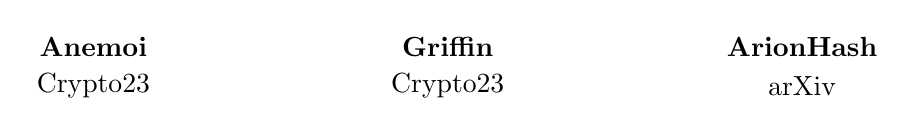
\begin{tikzpicture}[ultra thick,xscale=.9]
      \node (A1) at (0,0) {\bf Anemoi};
      \node (A2) at (0,-.5) {Crypto23};
      \node (B1) at (5,0) {\bf Griffin};
      \node (B2) at (5,-.5) {Crypto23};
      \node (C1) at (10,0) {\bf ArionHash};
      \node (C2) at (10,-.5) {arXiv};
    \end{tikzpicture}
  \end{center}

  \begin{itemize}
  \item Griffin, ArionHash and AnemoiSponge are Arithmetization-Oriented families of hash functions.
  \item Based on Griffin-$\pi$, Arion-$\pi$ and Anemoi families of permutations (all fixed-key block ciphers).

    \pause
  \item \textbf{Many} instances are defined: variable $\mathbb{F}_\p$, number of branches, exponents for monomial permutations...

    \begin{center}
      \textcolor{myred}{$\implies$ We attack some instance better than others.}
    \end{center}

  \end{itemize}
\end{frame}


\begin{frame}
  \frametitle{Griffin-$\pi$ - Round Function (4 branches)}
  \begin{figure}
    \centering
    \includegraphics[width=.9\textwidth]{./figures/griffin-round.png}
  \end{figure}

  \vspace{25pt}
  \end{frame}

\begin{frame}
  \frametitle{Griffin-$\pi$ - Round Function (4 branches)}
  \begin{figure}
    \centering
    \includegraphics[width=.9\textwidth]{./figures/griffin-round-inv.png}
  \end{figure}

  \begin{center}
    \textcolor{myred}{$\cdot^{1/\alpha}$ is the only high-degree operation} $\implies$ add one variable per $\cdot^{1/\alpha}$. 
  \end{center}
\end{frame}




\begin{frame}
  \frametitle{Griffin-$\pi$ - Model}
  \begin{itemize}
  \item \textbf{CICO problem}: $\mathcal{G}_\pi(\cdots || 0) = (\cdots || 0)$.

    $\implies$ One variable $\textcolor{olive}{x_0}$ in the input. One equation for the output (last branch at 0).
  \item $N_{rounds}$ equations of the form $\textcolor{purple}{x_i^\alpha} = P_i(\textcolor{olive}{x_0}, \textcolor{purple}{x_1}, \ldots \textcolor{purple}{x_{i-1}})$ $\quad$ ($\cdot^{1/\alpha}$ S-boxes).
  \end{itemize}

  \pause
  \begin{exemple}[$\alpha = 3$, one round]
    \vspace{-20pt}
    \begin{align*}
      &\textcolor{purple}{x_1^3} = a\textcolor{olive}{x_0} + b \\
      &\textcolor{olive}{x_0^7} + c\textcolor{olive}{x_0^4}\textcolor{purple}{x_1} + d\textcolor{olive}{x_0}\textcolor{purple}{x_1^2} + \cdots = 0
    \end{align*}

  \end{exemple}
\end{frame}





\begin{frame}
  \frametitle{Generic System Solving}

  \begin{tabular}{cccc}
    \onslide<1->{$\left\{
    \begin{aligned}
      p_1(\textcolor{mylb1}{x_1},\ldots&,\textcolor{myred}{x_N}) = 0 \\
      \vdots& \\
      p_{k-1}(\textcolor{mylb1}{x_1},\ldots&,\textcolor{myred}{x_N}) = 0 \\
      p_k(\textcolor{mylb1}{x_1},\ldots&,\textcolor{myred}{x_N}) = 0
    \end{aligned}
    \right.$}
    &
      \only<1>{$\left\{
      \begin{aligned}
        g_1(\textcolor{mylb1}{x_1},\ldots&,\textcolor{myred}{x_N}) = 0 \\
        \vdots& \\
        g_{\kappa-1}(\textcolor{mylb1}{x_1},\ldots&,\textcolor{myred}{x_N}) = 0 \\
        g_\kappa(\textcolor{mylb1}{x_1},\ldots&,\textcolor{myred}{x_N}) = 0
    \end{aligned}
      \right.$}\only<2>{\textcolor{gray}{$\left\{
      \begin{aligned}
        g_1(\textcolor{gray}{x_1},\ldots&,\textcolor{gray}{x_N}) = 0 \\
        \vdots& \\
        g_{\kappa-1}(\textcolor{gray}{x_1},\ldots&,\textcolor{gray}{x_N}) = 0 \\
        g_\kappa(\textcolor{gray}{x_1},\ldots&,\textcolor{gray}{x_N}) = 0
    \end{aligned}
      \right.$}}
    &
      \onslide<1->{$\left\{
      \begin{aligned}
        &g_1^*(\textcolor{mylb1}{x_1},\ldots,\textcolor{myred}{x_N}) = 0 \\
        &\hspace{1cm}\vdots \\
        &g_{N-1}^*(x_{N-1}, \textcolor{myred}{x_N}) = 0 \\ 
        &g_N^*(\textcolor{myred}{x_N}) = 0
    \end{aligned}
      \right.$}

      \medskip
    \\
    \onslide<1->{1. Define system} & \only<1>{2. Find a GB (F4/F5)}\only<2>{\textcolor{gray}{2. Find a GB (F4/F5)}} & \onslide<1->{3. Change order to \textbf{lex} (FGLM)}
                       
  \end{tabular}

  \medskip

  4. Find the roots in $\mathbb{F}_\q$ of $g_N^*$ with univariate methods, etc.

  \medskip

  Designers of Anemoi and Griffin base their security on the hardness of \textbf{Step 2}.

  \pause
  \begin{center}
    \textcolor{myred}{But we can skip it!}
    
    \vspace{-5.3cm}\hspace{-1.6cm}
\begin{tikzpicture}
    \draw[color=myred,line width=.2cm] (0,0) -- (3,3);
    \draw[color=myred,line width=.2cm] (0,3) -- (3,0);
    \end{tikzpicture}
  \end{center}


  
\end{frame}





\subsection{Using Weighted Orders}

\begin{frame}
  \frametitle{Griffin-$\pi$ - Model}
  \begin{itemize}
  \item \textbf{CICO problem}: $\mathcal{G}_\pi(\cdots || 0) = (\cdots || 0)$.

    $\implies$ One variable $\textcolor{olive}{x_0}$ in the input. One equation for the output (last branch at 0).
  \item $N_{rounds}$ equations of the form $\textcolor{purple}{x_i^\alpha} = P_i(\textcolor{olive}{x_0}, \textcolor{purple}{x_1}, \ldots \textcolor{purple}{x_{i-1}})$ $\quad$ ($\cdot^{1/\alpha}$ S-boxes).
  \end{itemize}

  \begin{exemple}[$\alpha = 3$, one round]
    \vspace{-20pt}
    \begin{align*}
      &\textcolor{purple}{x_1^3} = a\textcolor{olive}{x_0} + b \\
      &\textcolor{olive}{x_0^7} + c\textcolor{olive}{x_0^4}\textcolor{purple}{x_1} + d\textcolor{olive}{x_0}\textcolor{purple}{x_1^2} + \cdots = 0
    \end{align*}

    \pause
    
    \textbf{Observation}: $\textcolor{purple}{x_1}$ has a lower degree than $\textcolor{olive}{x_0}$ in the last equation.

    $\implies$ In \textbf{grevlex}, the leading monomials are $\textcolor{olive}{x_0^7}$ and $\textcolor{purple}{x_1^3}$.

    
    $\implies$ \textbf{It's a Gröbner basis} ! (coprime leading monomials)

    \pause
    
    For more rounds, \textbf{grevlex} doesn't work. We need \textbf{weighted degree} orders, with $\mathbf{wt}(\textcolor{olive}{x_0})=1$ and $\mathbf{wt}(\textcolor{purple}{x_i})=7^{i-1}$.
  \end{exemple}
\end{frame}


% \begin{frame}
%   \frametitle{Round of Griffin ($m=4$)}

%   \begin{figure}
%     \begin{center}
%       \input{griffin}
%     \end{center}
%     % \caption{One round of \textsc{Griffin} for $m = 4$. $Q_2$ and $Q_3$ are quadratic functions.}
%   \end{figure}

% \end{frame}

% \begin{frame}
%   \frametitle{Griffin Model and Free GB}

%   \begin{tabular}{cc}
%     \input{griffin-model}
%     & test
%   \end{tabular}
% \end{frame}


\begin{frame}
  \frametitle{Arion-$\pi$ - Round Function (4 branches)}
  \begin{figure}
    \centering
    \includegraphics[width=\textwidth]{./figures/arion-round.png}
  \end{figure}

  \vspace{25pt}
  \end{frame}

\begin{frame}
  \frametitle{Arion-$\pi$ - Round Function (4 branches)}
  \begin{figure}
    \centering
    \includegraphics[width=\textwidth]{./figures/arion-round-inv.png}
  \end{figure}

  \begin{center}
    \textcolor{myred}{$\cdot^{1/\alpha}$ is the only high-degree operation} $\implies$ add one variable per $\cdot^{1/\alpha}$. 
  \end{center}
\end{frame}


% \begin{frame}
%   \frametitle{Arion-$\pi$ - Model}
%   \begin{itemize}
%   \item \textbf{CICO problem}: $\mathcal{G}_\pi(\cdots || 0) = (\cdots || 0)$.

%     $\implies$ One variable $\textcolor{olive}{x_0}$ in the input. One equation for the output (last coordinate $= 0$).
%   \item $N_{rounds}$ equations of the form $\textcolor{purple}{x_i^\alpha} = P_i(\textcolor{olive}{x_0}, \textcolor{purple}{x_1}, \ldots \textcolor{purple}{x_{i-1}})$ $\quad$ ($\cdot^{1/\alpha}$ S-boxes).
%   \end{itemize}

%   \pause
%   \begin{exemple}[$\alpha = 121$, $e=3$, 4 branches, one round]
%     \vspace{-20pt}
%     \begin{align*}
%       &\textcolor{purple}{x_1^{121}} = a\textcolor{oflive}{x_0} + b \\
%       &\textcolor{olive}{x_0^{29}} + c\textcolor{olive}{x_0^4}\textcolor{purple}{x_1} + d\textcolor{olive}{x_0}\textcolor{purple}{x_1^2} + \cdots = 0
%     \end{align*}

%     \pause

%     \textbf{Observation}: $\textcolor{purple}{x_1}$ has a lower degree than $\textcolor{olive}{x_0}$ in the last equation.

%     $\implies$ In \textbf{grevlex}, the leading monomials are $\textcolor{olive}{x_0^7}$ and $\textcolor{purple}{x_1^3}$.
%     $\implies$ \textbf{It's a Gröbner basis} ! (coprime leading monomials)

%     $\implies$ For more rounds, \textbf{grevlex} doesn't work. We need \textbf{weighted degree} orders, with $\mathbf{wt}(\textcolor{olive}{x_0})=1$ and $\mathbf{wt}(\textcolor{purple}{x_i})=7^{i-1}$.
%   \end{exemple}
% \end{frame}


\subsection{The Case of Anemoi}

\begin{frame}
  \frametitle{Anemoi - Nonlinear layer (2 branches)}

  \definecolor{colorQi}{HTML}{FDC1C1}
  \definecolor{colorE-1}{HTML}{C1C1FD}
  \definecolor{colorQf}{HTML}{FDC1E1}
  \begin{center}
    \begin{tikzpicture}[xscale=0.8, yscale=0.4]
      \scriptsize
      % variables
      \draw (-3, 3) node(x){} ;
      \draw (+3, 3) node(y){} ;
      \draw[inner sep=0] (-3, -3) node(t){} ;
      \draw (-3, -9) node(u){} ;
      \draw (-2.5, -10.5) node{};
      \draw (+3, -9) node(v){} ;
      % boxes and additions
      % \draw[fill=colorQi!40] (-1, -1) rectangle (1, 1) node[pos=0.5]{$\beta x^{2} + \gamma$} ;
      \fill[fill=colorQi!70, rounded corners=2pt] (-1.25, -1.15) rectangle (1.25, 1.15) node[pos=0.5]{$F_1$} ;
      \draw (-3, 0) node[inner sep=0](add0){$\boxminus$} ;
      \fill[fill=colorE-1!70, rounded corners=2pt] (-1.25, -4.15) rectangle (1.25, -1.85) node[pos=0.5]{$(\cdot)^{1/\alpha}$} ;
      \draw (+3, -3) node[inner sep=0](add1){$\boxminus$} ;
      % \draw[fill=colorQf!40] (-1, -7) rectangle (1, -5) node[pos=0.5]{$\beta x^{2} + \delta$} ;
      \fill[fill=colorQf!70, rounded corners=2pt] (-1.25, -7.15) rectangle (1.25, -4.85) node[pos=0.5]{$F_2$} ;
      \draw (-3, -6) node[inner sep=0](add2){$\boxplus$} ;
      % arrows
      \draw[->] (x) -- (add0) ;
      \draw[->] (y) -- (add1) ;
      \draw[->] (3, 0) -- (1.25, 0) ;
      \draw[->] (-1.25, 0) -- (add0) ;
      \draw[->] (add0) -- (add2) ;
      \draw[->] (t) -- (-1.3, -3) ;
      \draw[->] (1.25, -3) -- (add1) ;
      \draw[->] (add1) -- (v) ;
      \draw[->] (3, -6) -- (1.25, -6) ;
      \draw[->] (-1.25, -6) -- (add2) ;
      \draw[->] (add2) -- (u) ;

    \end{tikzpicture}
  \end{center}
  
  % \begin{figure}
  %   \centering
  %   \includegraphics[width=.4\textwidth]{anemoi-round.png}
  % \end{figure}

  \vspace{25.3pt}
\end{frame}

\begin{frame}
  \frametitle{Anemoi - Nonlinear layer (2 branches)}

\definecolor{colorQi}{HTML}{FDC1C1}
  \definecolor{colorE-1}{HTML}{C1C1FD}
  \definecolor{colorQf}{HTML}{FDC1E1}
  \begin{center}
    \begin{tikzpicture}[xscale=0.8, yscale=0.4]
      \scriptsize
      % variables
      \draw (-3, 3) node(x){} ;
      \draw (+3, 3) node(y){} ;
      \draw[inner sep=0] (-3, -3) node(t){} ;
      \draw (-3, -9) node(u){} ;
      \draw (-2.5, -10.5) node{};
      \draw (+3, -9) node(v){} ;
      % boxes and additions
      % \draw[fill=colorQi!40] (-1, -1) rectangle (1, 1) node[pos=0.5]{$\beta x^{2} + \gamma$} ;
      \fill[fill=colorQi!70, rounded corners=2pt] (-1.25, -1.15) rectangle (1.25, 1.15) node[pos=0.5]{$F_1$} ;
      \draw (-3, 0) node[inner sep=0](add0){$\boxminus$} ;
      \fill[fill=colorE-1!70, rounded corners=2pt] (-1.25, -4.15) rectangle (1.25, -1.85) node[pos=0.5](sbox){$(\cdot)^{1/\alpha}$} ;
      \draw (+3, -3) node[inner sep=0](add1){$\boxminus$} ;
      % \draw[fill=colorQf!40] (-1, -7) rectangle (1, -5) node[pos=0.5]{$\beta x^{2} + \delta$} ;
      \fill[fill=colorQf!70, rounded corners=2pt] (-1.25, -7.15) rectangle (1.25, -4.85) node[pos=0.5]{$F_2$} ;
      \draw (-3, -6) node[inner sep=0](add2){$\boxplus$} ;
      % arrows
      \draw[->] (x) -- (add0) ;
      \draw[->] (y) -- (add1) ;
      \draw[->] (3, 0) -- (1.25, 0) ;
      \draw[->] (-1.25, 0) -- (add0) ;
      \draw[->] (add0) -- (add2) ;
      \draw[->] (t) -- (-1.3, -3) ;
      \draw[->] (1.25, -3) -- (add1) ;
      \draw[->] (add1) -- (v) ;
      \draw[->] (3, -6) -- (1.25, -6) ;
      \draw[->] (-1.25, -6) -- (add2) ;
      \draw[->] (add2) -- (u) ;

      \node[draw,dashed,circle,color=myred,thick,minimum size=1cm] at (sbox) {};

    \end{tikzpicture}
  \end{center}
  
  \begin{center}
    \textcolor{myred}{$(\cdot)^{1/\alpha}$ is the only high-degree operation} $\implies$ add one variable per $(\cdot)^{1/\alpha}$. 
  \end{center}
\end{frame}




\begin{frame}
  \frametitle{Anemoi - Model}
  % \begin{itemize}
  % \item \textbf{CICO problem}: $\mathcal{G}_\pi(\cdots || 0) = (\cdots || 0)$.

  %   $\implies$ One variable $\textcolor{olive}{x_0}$ in the input. One equation for the output (last branch at 0).
  % \item $N_{rounds}$ equations of the form $\textcolor{purple}{x_i^\alpha} = P_i(\textcolor{olive}{x_0}, \textcolor{purple}{x_1}, \ldots \textcolor{purple}{x_{i-1}})$ $\quad$ ($\cdot^{1/\alpha}$ S-boxes).
  % \end{itemize}

  % \pause
  \begin{exemple}[$\alpha = 3$, one round]
    {\small
    \vspace{-20pt}
    \begin{align*}
      &\textcolor{purple}{x_1^3} = a\textcolor{olive}{x_0^2} + b\textcolor{olive}{x_0} + c \\
      &\textcolor{olive}{x_0}\textcolor{purple}{x_1} + d\textcolor{purple}{x_1^2} + e\textcolor{olive}{x_0} + f\textcolor{purple}{x_1} + g  = 0
    \end{align*}
    }
  \end{exemple}

    \pause

    $\textcolor{olive}{x_0^2}$ cancels out: this isn't a Gröbner basis for any order!

    \pause

    \begin{exampleblock}{Saving the Freelunch}
      {\small 
        \textbf{Solution:} multiply last equation by $\textcolor{purple}{x_1^2}$ and reduce it by the first equation. We get:
        \[ p^*(\textcolor{olive}{x_0}, \textcolor{purple}{x_1}) = a\textcolor{olive}{x_0^3} + bd\textcolor{olive}{x_0^2}\textcolor{purple}{x_1} + \cdots \] 

        \pause
        $\implies$ The first equation and $p^*$ are a Gröbner basis for some weighted order.

        \pause

        This adds a few parasitic solutions (corresponding to $\textcolor{purple}{x_1}=0$), but not many.
      }
    \end{exampleblock}
\end{frame}


% \begin{frame}
%   \frametitle{Bypassing the First Rounds}
  
% \end{frame}

% \begin{frame}
%   \frametitle{Gröbner basis Cryptanalysis - What Remains}
%   Basically... FGLM and univariate solving
% \end{frame}



\subsection{Solving the System given a Gröbner Basis}

\begin{frame}
  \frametitle{FGLM in a Nutshell}

  \begin{itemize}
  \item Given a zero-dimensional ideal $\textcolor{myor}{I}$, a Gröbner basis $G_1$ for $\textcolor{myor}{I}$ some ordering $<_1$, and an ordering $<_2$, FGLM computes a Gröbner basis $G_2$ for $<_2$ in $O(n_{var}D_{\textcolor{myor}{I}}^3)$.
  \item $D_{\textcolor{myor}{I}}$ is the degree of the ideal, a.k.a. the number of \textbf{solutions of the system} in the algebraic closure.
    \pause
  \item \textbf{This is interesting} because a GB in \textbf{lex} order \textbf{must have} a univariate polynomial in the smallest variable, which we can solve. (This corresponds to eliminating the other variables.)

    \pause
  \item Free Gröbner basis, FGLM and symmetric techniques to bypass the first rounds is already enough to break some instances of Griffin and Arion.
  \end{itemize}
\end{frame}

\begin{frame}
  \frametitle{Faster Change of Order Strategy}
  \begin{itemize}
  \item Idea from a 2022 paper by Jérémy Berthomieu, Vincent Neiger, Mohab Safey El Din.
    
  \item Strategy: for the smallest variable $\textcolor{olive}{x}$, compute the characteristic polynomial $\chi$ of the linear operation $P \mapsto \text{Red}_<(\textcolor{olive}{x} \cdot P, G)$.

  \item $\chi(\textcolor{olive}{x})=0$. Generically, this is \textbf{exactly} the univariate polynomial in $\textcolor{olive}{x}$ in the reduced GB of ${\textcolor{myor}{I}}$ in \textbf{lex} order.

  \item \textbf{Issue:} our systems \textbf{do not} verify an important property of the original paper.
  \end{itemize}
\end{frame}


\begin{frame}
  \frametitle{Computing the Multiplication Matrix}

  \textbf{Step 1:} Compute the matrix $T$ of the linear operation in $\mathbb{F}[\textcolor{olive}{x_0},\textcolor{purple}{x_1},\ldots,\textcolor{purple}{x_N}]$ that maps $P$ to $\textcolor{olive}{x_0} \cdot P$.

  \begin{itemize}
  \item Need to reduce monomials of the form $\textcolor{olive}{x_0^{k_0+1}}\textcolor{purple}{x_1^{k_1}}\cdots \textcolor{purple}{x_N^{k_N}}$. \textbf{We have no tight complexity estimate for this step}.

    \pause
  \item The matrix is sparse. If leading monomials are $\textcolor{olive}{x_0^{d_0}},\ldots,\textcolor{purple}{x_N^{d_N}}$:
  \end{itemize}
  \begin{center}
    \includegraphics[width=8cm]{./figures/matrix}
  \end{center}
%   \[
%     T_0 = 
%     \begin{array}{cccc|c}%{w{c}{1cm}w{c}{1cm}w{c}{1cm}w{c}{1cm}|w{c}{1cm}}
%       0 & 0 & \cdots & 0 & * \\
%       \hline
%       1 & 0 & \cdots &  0 & * \\
%       0 & \cdots & \cdots & \cdots & \Vdots \\
%       \Vdots & \Ddots & \Ddots & 0 & \Vdots \\
%       0 & \Cdots & 0 & 1 & *
%       \CodeAfter
%       \UnderBrace[yshift=5pt]{1-1}{5-4}{\textcolor{olive}{(d_0-1)}\textcolor{purple}{d_1\cdots d_N}}
%       \UnderBrace[yshift=5pt]{1-5}{5-5}{\textcolor{purple}{d_1\cdots d_N}}
% \end{array}
% \]

  
\end{frame}

\begin{frame}
  \frametitle{Computing the Characteristic Polynomial}
  \textbf{Step 2:} Given $T$, compute $\text{det}(\textcolor{olive}{X}I - M)$.

  $\implies$ $T$ is sparse. With block matrix reasoning, this reduces to computing the determinant of a polynomial matrix of size $D_1 = \textcolor{purple}{d_1\cdots d_N}$.

  $\implies$ In Griffin and Arion, $\textcolor{olive}{d_0}$ is by far the highest degree, so this reduces complexity by a lot.

  $\implies$ This can be computed with fast linear algebra, in $\mathcal{O}(\textcolor{olive}{d_0}\text{log}(\textcolor{olive}{d_0})^2\textcolor{purple}{d_1^\omega\cdots d_N^\omega})$.

  
\end{frame}

% \section[Results]{Experimental and Theoretical Results}


\begin{frame}
  \frametitle{Our Full Algorithm}

  \begin{enumerate}
    \setlength\itemsep{0.3cm}
  \item \texttt{sysGen}: Compute the Freelunch system and the order for a free Gröbner basis.
  \item \texttt{matGen}: Compute the multiplication matrix $T$. \textbf{Complexity hard to evaluate}.
  \item \texttt{polyDet}: Compute the characteristic polynomial $\chi$ of $T$.

    $\implies$ \textbf{Longest step aside from} \texttt{matGen}.
  \item \texttt{uniSol}: Find roots of $\chi$ with Berlekamp-Rabin in $\mathcal{O}(D_{\textcolor{myor}{I}}\text{log}(D_{\textcolor{myor}{I}})\text{log}(\p D_{\textcolor{myor}{I}}))$.
  \end{enumerate}

\end{frame}



\begin{frame}
  \frametitle{Experimental Results}

  \begin{figure}
    \centering
    \includegraphics[width=.9\textwidth]{./figures/complexite-griffin-anemoi.png}

    \caption{\hspace{20pt} Complexity of Griffin  \hspace{105pt} Complexity of Anemoi \\ \hspace{45pt} (7 out of 10 rounds, $\alpha$=3) \hspace{83pt} (7 out of 21 rounds, $\alpha=3$)}
  \end{figure}

  \pause
  $\implies$ For Griffin, \texttt{polyDet} upper-bounds the others up to 7 rounds.

  $\implies$ For Anemoi, \texttt{matGen} is the bottleneck.
  
\end{frame}


\section{Combining an Root Finding with Other Techniques}


\begin{frame}{Skipping Rounds}
  \vfill

  \begin{center}
    \includegraphics[width=8cm]{./figures/simpsons}
  \end{center}
  
  \vfill
\end{frame}



\begin{frame}
  \frametitle{Conclusion}

  \begin{itemize}
  \item AO primitives \alert{should not} base their security on the complexity of finding a Gröbner basis (F4/F5).

  \item Instead, focus on the growth of $D_{\textcolor{myor}{I}}$ with the number of rounds (impacts the complexity of solving algorithms).

  \item \alert{Anemoi, Griffin and Arion need to recompute their numbers of rounds!}
  \end{itemize}

  \pause

  {\small
    \begin{exampleblock}{\texttt{MatGen} and \texttt{PolyDet} are already getting obsolete!}
      \begin{center}
        {\large Improved Resultant Attack against Arithmetization-Oriented Primitives}

        \vspace{0.2cm}
        \url{https://eprint.iacr.org/2025/259}

        
        \emph{Augustin Bariant, Aurélien Boeuf, Pierre Briaud, Maël Hostettler,\\ Morten Øygarden, Håvard Raddum}
      \end{center}
    \end{exampleblock}
  }
  
  \pause

  \centering
  {\textbf{Thank you!}}

\end{frame}

\appendix


\begin{frame}
  \frametitle{Griffin Trick}
  \begin{figure}
    \centering
    \includegraphics[height=.9\textheight]{./figures/griffin-trick.png}
  \end{figure}
\end{frame}

\begin{frame}
  \frametitle{Arion Trick}
  \begin{figure}
    \centering
    \includegraphics[height=.9\textheight]{./figures/arion-trick.png}
  \end{figure}
\end{frame}



\end{document}
